\documentclass[12pt]{article}
\usepackage[a4paper,top=2cm,bottom=2cm,left=1.5cm,right=1.5cm]{geometry}
\usepackage[utf8]{vietnam}
\usepackage{graphicx}
\usepackage{wrapfig}
\usepackage{float}
\usepackage{subcaption}
\usepackage{amsfonts,amsmath,amssymb}
\usepackage{siunitx}
\usepackage[hidelinks]{hyperref}
\usepackage{indentfirst}

%%%%%%%%%% DEFINE COLOR %%%%%%%%%%
\usepackage{xcolor} 
\definecolor{charcoal-blue}{RGB}{44, 64, 89}

%%%%%%%%%% EQUATION COUNTER & REFERENCE %%%%%%%%%% 
\usepackage{xassoccnt}
\newcounter{totalequations}
\DeclareAssociatedCounters{equation}{totalequations}
\let\theOldHequation\theHequation
\renewcommand{\theHequation}{\theOldHequation::\number\value{totalequations}}

%%%%%%%%%% PAGESTYLE %%%%%%%%%%
\usepackage{fancyhdr}
\pagestyle{fancy}
\fancyhf{}
\fancyhead[L]{\href{https://www.facebook.com/physicspen1111/}{
\includegraphics[width=0.15\textwidth]{Figures/Logo 2.png}}}
\fancyhead[R]{\color{charcoal-blue}{\vspace{0.05cm}\fontsize{13}{18}\selectfont\textbf{Switzerland 2025 - Chung kết}}}
\fancyfoot[C]{\thepage}
\setlength{\headsep}{30pt}


\begin{document}

%%%%%%%%%% FIRST PAGE STYLE %%%%%%%%%%
\thispagestyle{plain}

%%%%%%%%%% TITLE %%%%%%%%%%
\begin{center}
  \fontfamily{cmss}\fontseries{b}\LARGE{\textbf{Đề thi và Lời giải\\
      Olympic Vật lý Thuỵ Sĩ năm 2025\\
      Vòng Chung kết}}
\end{center}


%%%%%%%%%% PROBLEMS %%%%%%%%%%
\subsection*{Câu 1: Đĩa Faraday}
\noindent Đĩa Faraday là một máy phát điện đơn giản, có cấu tạo bao gồm một đĩa kim loại làm bằng sắt (một loại vật liệu dẫn điện) có bán kính trong là $r_1$, bán kính ngoài là $r_2$ và độ dày là $h$. \\
\begin{figure}[H]
  \centering
  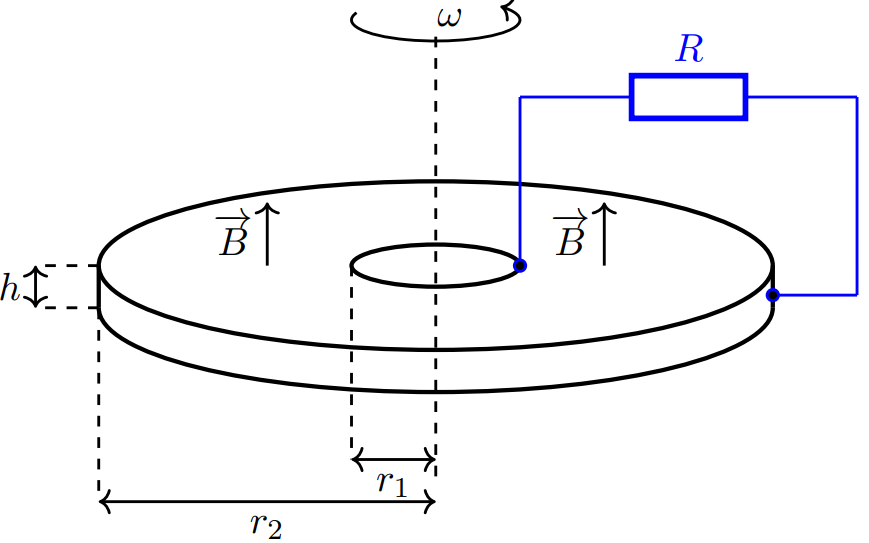
\includegraphics[width=0.5\textwidth]{Figures/Problems/Fig 1.1.png}
  \begin{center}
    \figurename{ 1}
  \end{center}
\end{figure}
\vspace{-0.5cm}
\noindent Đĩa được đặt trong một từ trường đều không đổi có cảm ứng từ $\vec{B}$ theo phương vuông góc với mặt phẳng của đĩa như được biểu diễn trong hình vẽ. Độ dẫn điện của sắt là $\sigma$.

\subsubsection*{Phần A: Mạch hở}
\noindent Trong phần này, người ta cho đĩa quay với tốc độ góc không đổi $\omega$ như Hình 1. Lúc này, đĩa chưa được nối với điện trở $R$ (không có đoạn mạch màu xanh dương).
\begin{enumerate}
  \item Xác định điện trường $\vec{E}$ bên trong đĩa và hiệu điện thế $V_0$ giữa mép trong và mép ngoài của đĩa. \textit{Gợi ý:} Trong một vật dẫn ở trạng thái cân bằng tĩnh điện, hợp lực tác dụng lên các điện tích tự do bằng không.
  \item Tìm điện trở $R_0$ của đĩa.
\end{enumerate}

\subsubsection*{Phần B: Phát điện}
\noindent Bây giờ, mép trong và mép ngoài của đĩa được nối với một điện trở $R$ như được minh họa bằng màu xanh dương trong hình vẽ. Các tiếp điểm không quay cùng với đĩa. Giả sử các tiếp điểm không có điện trở. Bỏ qua mọi ma sát.
\begin{enumerate}
  \item Xác định hiệu điện thế $V$ giữa mép trong và mép ngoài của đĩa. \textit{Gợi ý:} Lúc này, đĩa hoạt động như một nguồn điện không lý tưởng.
  \item Tính tổng công suất $P_0$ và công suất điện $P$ của nguồn.
  \item Tìm hiệu suất $\eta$ của máy phát.
  \item Tìm công suất điện cực đại $P_{\text{max}}$ và hiệu suất của nguồn khi hoạt động tại công suất đầu ra này.
\end{enumerate}

\subsubsection*{Phần C: Phanh tái sinh}
\noindent $N$ đĩa Faraday được dùng làm bánh xe và được kết nối cơ học với một đoàn tàu. Đoàn tàu có khối lượng $M = 400$ tấn và điện trở hiệu dụng $R$, mỗi bánh xe có khối lượng $m = 30$ kg. Phần duy nhất của tàu có chuyển động quay là các bánh xe. Sắt có độ dẫn điện $\sigma = 1{,}0 \cdot 10^7~\Omega^{-1} \cdot m^{-1}$, nhiệt dung riêng $c = 4{,}5 \cdot 10^2~J\,kg^{-1}\,K^{-1}$ và nhiệt độ nóng chảy $T = 1800~\text{K}$.
\begin{enumerate}
  \item Biểu diễn động năng của đoàn tàu dưới dạng $E = \frac{1}{2}I_{\text{eff}}\omega^2$ theo các đại lượng đã cho khi bánh xe quay với tốc độ góc $\omega$. Tìm $I_{\text{eff}}$. \textit{Gợi ý:} Moment quán tính của một vành tròn có khối lượng $M$, bán kính trong $R_1$ và bán kính ngoài $R_2$ đối với trục quay đi qua tâm và vuông góc với mặt phẳng vành là
        \begin{equation*}
          \frac{1}{2} M(R_2^2 + R_1^2)
        \end{equation*}
  \item Xác định động năng của đoàn tàu trong trường hợp $M \gg Nm$.
  \item Trong các ý còn lại của phần C, bạn có thể giả sử rằng $M \gg Nm$.
  \item Xác định tốc độ góc $\omega$ tại thời điểm $t$.
  \item Mất bao lâu để tốc độ của tàu giảm đi một nửa?
  \item Nếu tàu được hãm bằng cách nối tắt vành trong với vành ngoài của đĩa (lúc này $R = 0$), hãy ước lượng số lượng bánh xe tối thiểu để chúng không bị nóng chảy.
  \item Gia tốc khi hãm phanh có an toàn cho hành khách không? Lấy $B = 0{,}1\,$T, $r_1 = 10\,$cm, $r_2 = 50\,$cm và $h = 1{,}0\,$cm.
\end{enumerate}

\subsection*{Câu 2: Quang học phi tuyến}
\begin{wrapfigure}{r}{9cm}
  \centering
  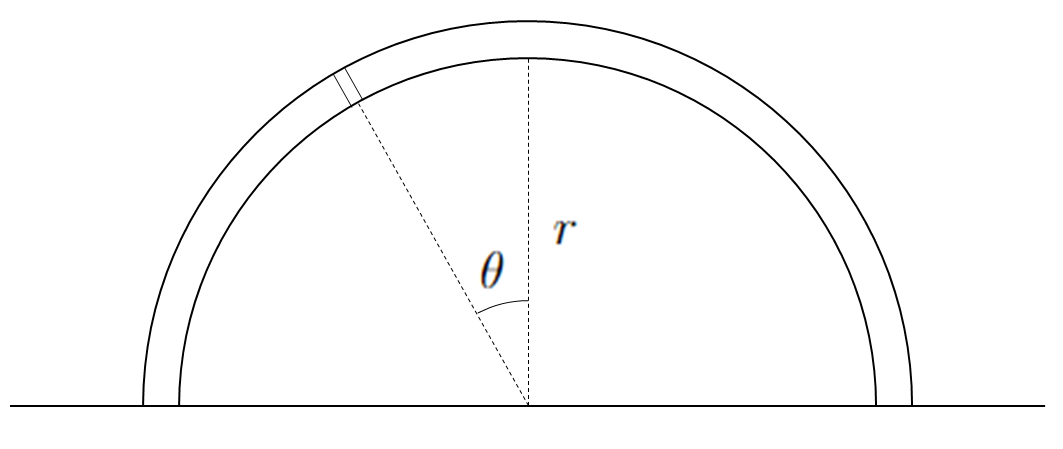
\includegraphics[width=0.5\textwidth]{images/Hinh 2.PNG}
  \vspace{-25px}
  \begin{center}
    \figurename{ 2}
  \end{center}
  \vspace{15px}
\end{wrapfigure}

\vspace{-30px}
\noindent Một ống thuỷ tinh mỏng, tiết diện đều, hai đầu bịt kín được uốn thành một nửa đường tròn bán kính $r$ (bán kính tiết diện của ống rất nhỏ so với $r$) sau đó được gắn cố định trên trên mặt sàn nằm ngang sao cho toàn bộ ống nằm trong mặt phẳng thẳng đứng như hình 2. Bên trong ống có một piston mỏng có khối lượng $m$ được làm bằng kim loại, diện tích của piston bằng với tiết diện của ống thuỷ tinh. Đường nối tâm đường tròn và vị trí của piston hợp với phương thẳng đứng một góc $\theta$. Hai bên piston đều chứa n mol khí lý tưởng, giả sử nhiệt độ của khí luôn bằng nhiệt độ $T$ của môi trường bên ngoài. Cho biết gia tốc trọng trường có độ lớn $g$, hằng số khí lý tưởng $R$, xem như tất cả các quá trình biến đổi trạng thái của khí đều chuẩn tĩnh. Bỏ qua mọi ma sát.\\
\vspace{-15pt}
\begin{enumerate}
  \item Khi nhiệt độ $T$ lớn hơn một nhiệt độ tới hạn $T_{C}$ nào đó, vị trí cân bằng bền của piston nằm ngay chính giữa ống ($\theta=0$). Hãy tìm biểu thức của $T_{C}$ và xác định tần số góc trong dao động bé của piston quanh vị trí cân bằng này.
  \item Khi $T=T_{C}$, hãy đánh giá tính ổn định của piston khi nó nằm cân bằng ở giữa ống ($\theta=0$).\\
\end{enumerate}
\vspace{-15px}
\noindent Đối với các câu hỏi bên dưới, xem $T_{C}$ như một thông số đã biết và không cần thay vào giá trị mà bạn đã tìm được ở ý 1.
\begin{enumerate}
  \setcounter{enumi}{2}
  \item Khi $T<T_{C}$, piston cân bằng tại vị trí góc $\theta_{0}$, tìm phương trình mà $\theta_{0}$ phải thoả mãn. Xác định biểu thức gần đúng khi nhiệt độ $T$ giảm nhẹ (xấp xỉ đến bậc thấp nhất khác 0).
  \item Khi $T<T_{C}$, xác định tần số góc $\omega_{0}$ trong dao động bé của piston quanh vị trí cân bằng tại $\theta_{0}$, tần số này bằng bao nhiêu khi nhiệt độ của khí lớn hơn và nhỏ hơn $T_{C}$ một chút.
  \item Khi $T<T_{C}$, giả sử vận tốc ban đầu của piston gần như bằng không, hãy tìm độ lớn vận tốc góc của piston khi nó di chuyển từ vị trí chính giữa $(\theta=0)$ đến vị trí góc lớn nhất $\theta$ mà nó có thể đi được.
\end{enumerate}

\subsection*{Câu 3: Dây và bàn}
\vspace{-1cm}
\begin{wrapfigure}[16]{r}{7cm}
  \centering
  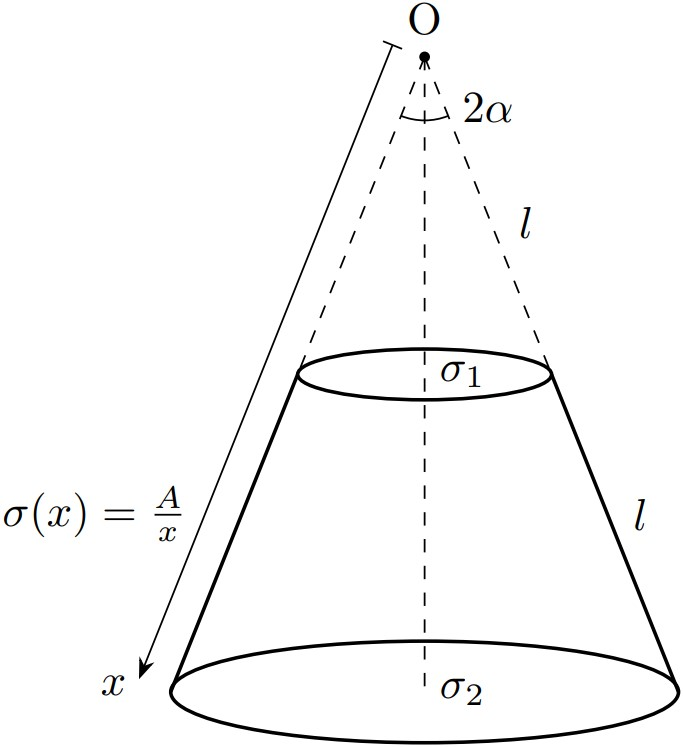
\includegraphics[width=0.38\textwidth]{Figures/Fig 3.jpg}
  \begin{center}
    \figurename{ 3}
  \end{center}
\end{wrapfigure}

\noindent Một khối đặc có dạng nón cụt, không dẫn điện, được tích điện trên mặt bên sao cho mật độ điện tích mặt thay đổi theo khoảng cách $x$ đến đỉnh $O$ theo công thức $\sigma(x)=A/x$ với $A$ là một hằng số dương đã biết. Đáy trên và đáy dưới của hình nón cụt được tích điện đều với mật độ điện tích tương ứng là $\sigma_{1}$ và $\sigma_{2}$. Độ dài đường sinh và nửa góc ở đỉnh của hình nón đầy đủ lần lượt là $2l$ và $\alpha=30^{\circ}$, độ dài đường sinh của hình nón cụt là $l$.
\begin{enumerate}
  \item Giả sử $\sigma_{1}=-\sigma_{2}=\sigma_{0}$ với $\sigma_{0}$ là một giá trị đã biết. Xác định độ lớn điện trường $E_{O}$ tại điểm $O$ trên hình 3.
\end{enumerate}
Bên trong hình nón cụt, người ta đục một lỗ nhỏ dọc theo trục đối xứng của nó. Một điện tích thử $-q$ với $q>0$, khối lượng $m$, có thể di chuyển không ma sát bên trong lỗ này. Giả sử $\sigma_{1}=\sigma_{2}=\sigma_{0}$.
\begin{enumerate}
  \setcounter{enumi}{1}
  \item Xác định khoảng cách từ vị trí cân bằng của điện tích thử bên trong hình nón cụt tới điểm $O$. Đồng thời, hãy chỉ ra rằng, khoảng cách này không phụ thuộc vào $\sigma_{0}$.
  \item Với giá trị nào của $\sigma_{0}$ thì cân bằng của điện tích thử ở vị trí vừa tìm được ở ý trên là bền? Tìm chu kỳ dao động bé của điện tích thử quanh vị trí cân bằng này.
\end{enumerate}
Trong suốt bài toán, hình nón cụt được giữ cố định. Cho biết hằng số điện môi của vật liệu làm nên hình nón cụt là $\varepsilon=1$, bỏ qua tác dụng của trọng lực và các hiện tượng từ tính.\\

\newpage
\quad\\
\begin{center}
  \vspace{-1cm}
  \noindent\LARGE\textbf{LỜI GIẢI THAM KHẢO}
\end{center}

\subsection*{Câu 1: Đĩa Faraday}
\noindent\textbf{1a.}
\begin{equation*}
  M=\frac{\pi r^{2}L}{2}(1+c)
\end{equation*}
\begin{equation*}
  d=\frac{\dfrac{\pi r^{2}L}{2}\left(\dfrac{4r}{3\pi}-\dfrac{4r}{3\pi}c\right)}{\dfrac{\pi r^{2}L}{2}(1+c)}=\frac{4r}{3\pi}\left(\frac{1-c}{1+c}\right)
\end{equation*}

\noindent\textbf{1b.} Momen quán tính của một khối trụ đặc có khối lượng $M$ và bán kính $r$ là $\dfrac{1}{2}Mr^2$ do đó
\begin{equation*}
  I=\frac{1}{2}\left(\frac{\pi r^{2}L}{2}\right)(1+c)r^{2}=\frac{\pi r^{4}L}{4}(1+c)
\end{equation*}

\noindent\textbf{2.} Định luật II Newton cho
\begin{equation*}
  \tau=I\ddot{\theta}
\end{equation*}
momen lực đối với trục đối xứng là
\begin{equation*}
  \begin{gathered}
    \tau=-Mgd\sin\theta \\
    I\ddot{\theta}=-Mgd\sin\theta \\
    \ddot{\theta}=-\frac{Mgd}{I}\sin\theta \\
    \Rightarrow T=\frac{2\pi}{\omega}=2\pi\sqrt{\frac{I}{Mgd}}
  \end{gathered}
\end{equation*}

\noindent\textbf{3a.} \\
\noindent\underline{\textbf{Cách 1}}: Phương trình chuyển động của khối trụ đối với trục quay đi qua điểm tiếp xúc
\begin{equation*}
  \tau=I_{\text{con}}\ddot{\theta}
\end{equation*}
momen lực tác dụng lên khối trụ tương tự như ý trên
\begin{equation*}
  \tau = -Mgd\sin\theta\approx - M g d \theta
\end{equation*}
momen quán tính đối với trục quay qua điểm tiếp xúc được cho bởi
\begin{equation*}
  I_{\text{con}}=I_{cm}+M(r-d)^{2}
\end{equation*}
\begin{equation*}
  I=I_{cm}+Md^{2}
\end{equation*}
\begin{equation*}
  \Rightarrow I_{\text{con}}=I+M((r-d)^{2}-d^{2})=I+M(r^{2}-2rd)
\end{equation*}
\begin{equation*}
  \Rightarrow\ddot{\theta}=-\frac{Mgd}{I_{con}}\theta
\end{equation*}
chu kì dao động
\begin{equation*}
  T=2\pi\sqrt{\frac{I_{con}}{Mgd}}=2\pi\sqrt{\frac{I+M(r^{2}-2rd)}{Mgd}}
\end{equation*}
có thể thấy, khi $d\rightarrow0$, chu kì $T\rightarrow0$.\\

\noindent\underline{\textbf{Cách 2}}: Hàm Lagrange là
\begin{equation*}
  L=T-U=\frac{1}{2}I_{con}\dot{\theta}^2-\frac{1}{2}Mgd\theta^2
\end{equation*}
phương trình chuyển động được cho bởi
\begin{equation*}
  \begin{gathered}
    \frac{d}{dt}\frac{\partial L}{\partial\theta}-\frac{\partial L}{\partial\theta}=0\Rightarrow I_{con}\ddot{\theta}+Mgd\theta=0 \\
    \Rightarrow\ddot{\theta}=-\frac{Mgd}{I_{con}}\theta                                                                           \\
    \Rightarrow T=2\pi\sqrt{\frac{I_{con}}{Mgd}}=2\pi\sqrt{\frac{I+M(r^{2}-2rd)}{Mgd}}
  \end{gathered}
\end{equation*}

\noindent\textbf{3b.} Vì khối trụ chỉ có thể lăn không trượt, năng lượng của nó là bảo toàn. Để thoát khỏi sự dao động, khối trụ phải có đủ động năng để khối tâm có thể lên đến vị trí thế năng cực đại
\begin{equation*}
  \frac{1}{2}Mv_{cm}^{2}+\frac{1}{2}I_{cm}\omega_{0}^{2}+Mg(r-d)=Mg(r+d)
\end{equation*}
\begin{equation*}
  \begin{gathered}
    \Rightarrow\frac{1}{2}M\omega_{0}^{2}(r-d)^{2}+\frac{1}{2}(I-Md^{2})\omega_{0}^{2}=2Mgd \\
    \Rightarrow\omega_{0}=\sqrt{\frac{4Mgd}{M(r-d)^{2}+(I-Md^{2})}}
  \end{gathered}
\end{equation*}
có thể thấy, khi $d\rightarrow0$, $\omega_0\rightarrow0$, điều này có nghĩa không có bất kì cân bằng bền nào trong giới hạn này và khối trụ sẽ tiếp tục di chuyển về một phía.\\

\subsection*{Câu 2: Quang học phi tuyến}
\noindent\textbf{1.1}
\begin{equation*}
  m = \rho V = \rho \cdot \left(\frac{\pi d^2}{4} \cdot h\right) = 9{,}6 \times 10^{-4}~\text{kg}
\end{equation*}

\noindent\textbf{1.2} Moment từ của nam châm có thể được tính thông qua định nghĩa của độ từ hóa:
\begin{equation*}
  M_R = \frac{p_m}{V} \quad \implies \quad p_m = M_R V
\end{equation*}
Sử dụng mối liên hệ đã cho giữa độ từ hóa và cảm ứng từ dư $B_R = \mu_0 M_R$, ta thu được:
\begin{equation*}
  p_m = \frac{B_R}{\mu_0} \cdot \left( \frac{\pi d^2}{4} \cdot h \right) = 0{,}14~\text{Am}^2
\end{equation*}

\noindent\textbf{1.3} Cường độ dòng điện từ hoá có thể được tính theo công thức moment từ:
\begin{equation*}
  p_m = I_m S \implies I_m = \frac{p_m}{S} = \left( \frac{B_R}{\mu_0} \right) \cdot \left( \frac{V}{S} \right) = \frac{B_R}{\mu_0} h = 1{,}1 \times 10^4~\text{A}
\end{equation*}

\noindent\textbf{2.1} Các thành phần của cảm ứng từ do từ tích điểm gây ra được xác định từ công thức:

\begin{equation*}
  B = \frac{\mu_0}{4\pi}\frac{q_m}{R^2}
\end{equation*}
kết hợp với hình vẽ ta được:
\begin{figure}[H]
  \centering
  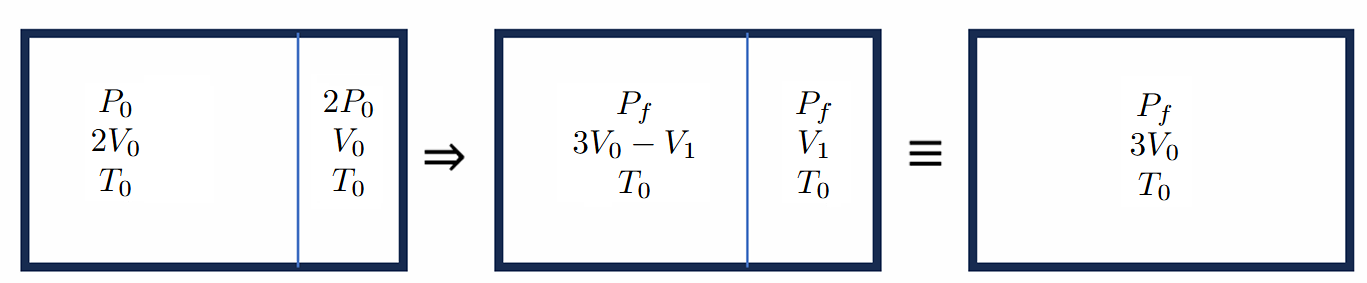
\includegraphics[width=0.2\textwidth]{Figures/Solutions/Fig 2.1.png}
\end{figure}

\begin{equation*}
  B^{(0)}_z(r, z)  = \frac{\mu_0}{4\pi}\frac{q_m}{R^2} \cos \alpha = \frac{\mu_0 q_m}{4\pi} \frac{z}{(r^2 + z^2)^{3/2}} \\
\end{equation*}
\begin{equation*}
  B^{(0)}_r(r, z)  = \frac{\mu_0}{4\pi}\frac{q_m}{R^2} \sin \alpha = \frac{\mu_0 q_m}{4\pi} \frac{r}{(r^2 + z^2)^{3/2}}
\end{equation*}

\noindent\textbf{2.2}\\
\begin{figure}[H]
  \centering
  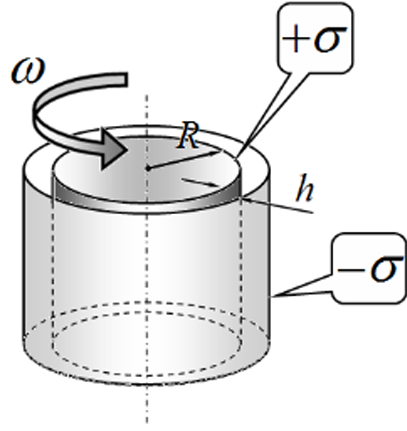
\includegraphics[width=0.3\textwidth]{Figures/Solutions/Fig 2.2.png}
\end{figure}

\noindent\textbf{2.3} Để giải phần này, ta có thể dùng gợi ý trong đề. Cách thứ hai là dùng nguyên lý chồng chất, viết biểu thức chính xác cho cảm ứng từ và khai triển theo tham số nhỏ $a$. Ở đây, ta sẽ sử dụng cách ngắn gọn hơn:
\begin{equation*}
  B_z(r, z) = B^{(0)}_z(r, z) - B^{(0)}_z(r, z + a) \approx -\left(B^{(0)}_z(r, z)\right)' \cdot a    \\
\end{equation*}
\begin{equation*}
  B_z(r, z)  = -\frac{\mu_0 q_m a}{4\pi} \cdot \frac{d}{dz} \left[ \frac{z}{(r^2 + z^2)^{3/2}} \right]  = \frac{\mu_0 p_m}{4\pi} \frac{2z^2 - r^2}{(r^2 + z^2)^{5/2}}
\end{equation*}

\noindent\textbf{2.4} Đồ thị định tính của hàm này có thể được vẽ thông qua các phân tích định tính: hàm là chẵn, bằng 0 tại $r = \pm \sqrt{2}z$, có các đoạn đơn điệu rõ ràng, tiệm cận về 0 khi $z \to \pm\infty$.\\
\begin{figure}[H]
  \centering
  \begin{subfigure}[b]{0.49\textwidth}
    \centering
    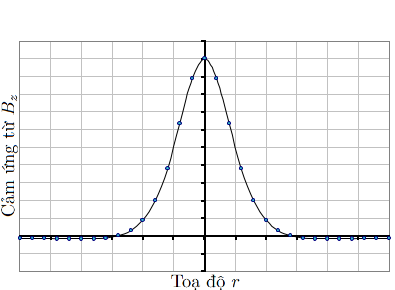
\includegraphics[width=0.9\textwidth]{Figures/Solutions/Fig 2.3.png}
  \end{subfigure}
  \hfill
  \begin{subfigure}[b]{0.49\textwidth}
    \centering
    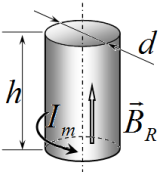
\includegraphics[width=0.6\textwidth]{Figures/Solutions/Fig 2.4.png}
  \end{subfigure}
\end{figure}


\noindent\textbf{2.5} Với $r = 0$ ta có:
\begin{equation*}
  B_z(z) = \frac{\mu_0 p_m}{4\pi} \frac{2z^2 - r^2}{(r^2 + z^2)^{5/2}} \Big|_{r = 0} = \frac{\mu_0 p_m}{2\pi z^3}
\end{equation*}

\noindent\textbf{2.6} Thực hiện tương tự:
\begin{equation*}
  B_r(r, z) = B^{(0)}_r(r, z) - B^{(0)}_r(r, z + a) = -\left(B^{(0)}_r(r, z)\right)' \cdot a
\end{equation*}
\begin{equation*}
  B_r(r, z) = -\frac{\mu_0 q_m a}{4\pi}  \left[ \frac{r}{(r^2 + z^2)^{3/2}} \right]'
  = \frac{\mu_0 p_m}{4\pi} \frac{3rz}{(r^2 + z^2)^{5/2}}
\end{equation*}

\noindent\textbf{2.7} Đồ thị của hàm này có thể được xây dựng trên cơ sở các phân tích định tính: hàm là lẻ, bằng 0 tại $z = 0$; có xu tiệm cận về 0 khi $z \to \pm \infty$.\\
\begin{figure}[H]
  \centering
  \begin{subfigure}[b]{0.49\textwidth}
    \centering
    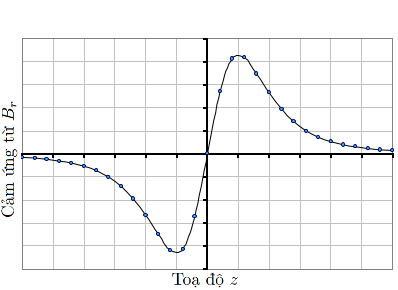
\includegraphics[width=0.9\textwidth]{Figures/Solutions/Fig 2.5.png}
  \end{subfigure}
  \hfill
  \begin{subfigure}[b]{0.49\textwidth}
    \centering
    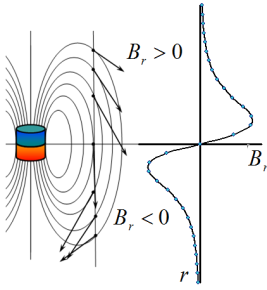
\includegraphics[width=0.6\textwidth]{Figures/Solutions/Fig 2.6.png}
  \end{subfigure}
\end{figure}


\noindent\textbf{2.8} Cảm ứng từ theo phương $r$ là cực đại khi:
\begin{equation*}
  \left(B_r(r, z)\right)'_z  = \frac{\mu_0 p_m}{4\pi}  3r \left( \frac{z}{(r^2 + z^2)^{5/2}} \right)'  = \frac{\mu_0 p_m}{4\pi}  3r  \frac{r^2 - 4z^2}{(r^2 + z^2)^{7/2}} = 0
\end{equation*}
Từ phương trình trên suy ra vị trí cực trị là $z^* = \pm \dfrac{r}{2}$. Giá trị cực đại là:
\begin{equation*}
  B_{r\text{max}}(r, z) = \frac{\mu_0 p_m}{4\pi} \frac{3rz}{(z^2 + r^2)^{5/2}} \Big|_{z = \frac{r}{2}}  = \frac{3}{2} \left( \frac{4}{5} \right)^{5/2} \frac{\mu_0 p_m}{4\pi r^3} = C  \frac{\mu_0 p_m}{r^3}
\end{equation*}
Trong đó:
\begin{equation*}
  C = \frac{3}{8\pi} \left( \frac{4}{5} \right)^{5/2} \approx 0{,}068
\end{equation*}

\begin{wrapfigure}[7]{r}{5.5cm}
  \centering
  \vspace{-0.5cm}
  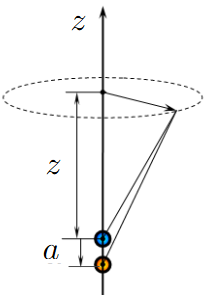
\includegraphics[width=0.28\textwidth]{Figures/Solutions/Fig 2.7.png}
\end{wrapfigure}
\noindent\textbf{3.1} Xét một lưỡng cực từ nằm trong một từ trường không đều $B(z)$. Hướng của moment lưỡng cực song song với hướng của trường từ. Khi đó, tổng lực tác dụng lên lưỡng cực là:
\begin{equation*}
  F = -q_m B(z) + q_m B(z + a)
\end{equation*}
Vì $a \ll z$, biểu thức có thể viết lại dưới dạng:
\begin{equation*}
  F \approx q_m a \cdot \frac{B(z + a) - B(z)}{a} = p_m B'(z)
\end{equation*}
Trong đó $B'(z)$ là đạo hàm của cảm ứng từ theo $z$. Ta có:
\begin{equation*}
  F = p_m \cdot \frac{d}{dz} \left( \frac{\mu_0 p_m}{2\pi z^3} \right) = -\frac{3\mu_0 p_m^2}{2\pi z^4}
\end{equation*}

\noindent\textbf{3.2} Với cách sắp xếp nam châm như trong hình a), lực từ cân bằng với trọng lực:
\begin{equation*}
  \frac{3\mu_0 p_m^2}{2\pi L^4} = mg
\end{equation*}
Từ đó suy ra khoảng cách cần tìm:
\begin{equation*}
  L = \left( \frac{3 \mu_0 p_m^2}{2\pi m g} \right)^{1/4}
\end{equation*}

\noindent\textbf{3.3} Chỉ có thể thực hiện thí nghiệm với phương án a), vì trạng thái cân bằng trong trường hợp này là bền. Cân bằng trong trường hợp b) là không bền.\\

\noindent\textbf{3.4} Thay giá trị số ta thu được:
\begin{equation*}
  L = 3{,}3~\text{cm}
\end{equation*}

\begin{wrapfigure}[11]{r}{5.5cm}
  \centering
  \vspace{-0.5cm}
  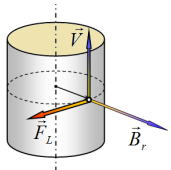
\includegraphics[width=0.28\textwidth]{Figures/Solutions/Fig 2.8.png}
\end{wrapfigure}
\noindent\textbf{4.1} Khi nam châm chuyển động, từ trường tại mỗi điểm trên thành ống sẽ biến thiên, từ đó sinh ra dòng điện cảm ứng, còn gọi là dòng Foucault.\\
\indent Để thuận tiện cho việc tính toán, ta sẽ sử dụng hệ quy chiếu gắn với nam châm. Trong hệ quy chiếu này, ống nhôm chuyển động trong từ trường. Nguồn của suất điện động (EMF) là lực Lorentz tác dụng lên điện tích dưới ảnh hưởng của thành phần xuyên tâm $B_r$ của cảm ứng từ. Lực Lorentz có phương này tiếp tuyến với thành ống và có độ lớn:
\begin{equation*}
  F_L = q V B_r
\end{equation*}
Suất điện động xuất hiện trong vòng dây ôm lấy ống là:
\begin{equation*}
  \varepsilon = \frac{1}{q} F_L \cdot 2\pi r_0 = 2\pi r_0 B_r V
\end{equation*}
Áp dụng định luật Ohm ta có:
\begin{equation*}
  \Delta I = \frac{\varepsilon}{R} = \frac{B_r V h_0 \Delta z}{\rho}
\end{equation*}
Cuối cùng:
\begin{equation*}
  \Delta I = \frac{B_{r,\text{max}} V h_0 \Delta z}{\rho}
\end{equation*}

\begin{wrapfigure}[7]{r}{4.5cm}
  \centering
  \vspace{-0.5cm}\hspace{-1cm}
  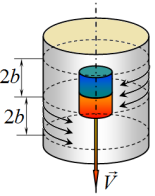
\includegraphics[width=0.2\textwidth]{Figures/Solutions/Fig 2.9.png}
\end{wrapfigure}
\noindent\textbf{4.2} Dòng điện xuất hiện ở tất cả các phần của ống nơi tồn tại từ trường xuyên tâm. Trong mô hình gần đúng “bậc thang”, thành phần xuyên tâm tồn tại trong một vùng có chiều rộng $4b$. Hướng của dòng điện không quan trọng vì công suất nhiệt không phụ thuộc vào hướng dòng. Vì vậy, ta có thể dùng biểu thức cho cường độ dòng điện hiệu dụng:
\begin{equation*}
  I = \frac{B_{r,\text{max}} V h_0}{\rho} \cdot 4b
\end{equation*}
Công suất toả nhiệt có thể được xác định thông qua định luật Joule–Lenz:
\begin{equation*}
  P = I^2 R
\end{equation*}
Trong đó $R = \rho \cdot \frac{2\pi r_0}{4b h_0}$ là điện trở phần thành ống nơi dòng điện chạy qua. Như vậy:
\begin{equation*}
  P = \left( \frac{B_{r,\text{max}} V h_0}{\rho} \cdot ab \right)^2 \cdot \frac{2\pi r_0}{4b h_0}   = \left( \frac{8\pi r_0 b h_0}{\rho} \right) B_{r,\text{max}}^2 V^2
\end{equation*}

\noindent\textbf{4.3} Công suất nhiệt tính được ở trên chính là công do lực ma sát từ sinh ra:
\begin{equation*}
  P = F \cdot V
\end{equation*}
Do đó, lực ma sát từ có độ lớn:
\begin{equation*}
  F = \left( \frac{8\pi r_0 b h_0}{\rho} \right) B_{r,\text{max}}^2 V
\end{equation*}

\noindent\textbf{4.4} Vận tốc của nam châm ổn định khi lực ma sát từ bằng với trọng lượng của nam châm:
\begin{equation*}
  \left( \frac{8\pi r_0 b h_0}{\rho} \right) B_{r,\text{max}}^2 V = mg \implies V = \frac{mg \rho}{8\pi r_0 b h_0 B_{r,\text{max}}^2}
\end{equation*}

\noindent\textbf{4.5}
\begin{equation*}
  B_{r,\text{max}} = C \frac{\mu_0 p_m}{r_0^3} \approx 0{,}45~\text{T}
\end{equation*}
\begin{equation*}
  V = \frac{mg \rho}{8\pi r_0 b h_0 B_{r,\text{max}}^2} \approx 3{,}9~\text{cm/s}
\end{equation*}




\subsection*{Câu 3: Dây và bàn}
\subsection*{Phần 1: Giới thiệu Toán học}
\noindent\textbf{1.} Để chứng minh công thức \eqref{eq:p31} ta cần sử dụng các phép xấp xỉ cho hàm mũ:
\begin{equation}
  \label{eq:31}
  \sqrt{a^{2} + x^{2}} = a \left( 1 + \frac{x^{2}}{a^{2}} \right)^{1/2} \approx a \left( 1 + \frac{x^{2}}{2a^{2}} \right) = a + \frac{x^{2}}{2a}
\end{equation}

\noindent\textbf{2.} Phương trình của đường tròn được mô tả có dạng:
\begin{equation}
  \label{eq:32}
  x^{2} + (y - R)^{2} = R^{2}
\end{equation}
sử dụng công thức \eqref{eq:p31} trong đề bài ta được:
\begin{equation}
  \label{eq:33}
  x^{2} + (y - R)^{2} = R^{2} \implies y - R = \pm \sqrt{R^{2} - x^{2}} \implies y = R - \frac{x^{2}}{2R}
\end{equation}

\subsection*{Phần 2: Sự đẳng thời}
\begin{wrapfigure}[11]{r}{6cm}
  \centering
  \vspace{-4mm}
  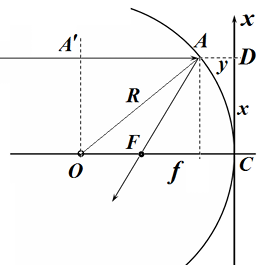
\includegraphics[width=0.3\textwidth]{Figures/P3/Fig 3.1S.png}
\end{wrapfigure}

\noindent\textbf{1.} Ta có thể xem tiêu điểm là ảnh của một điểm sáng nằm tại vô cùng. Theo nguyên lý đẳng thời cho sự  tạo ảnh, ta cần chứng minh rằng tồn tại một điểm $F$ mà  thời gian ánh sáng chuyển động đến $F$ là như nhau với mọi tia sáng. Do tính đối xứng, điểm này phải nằm trên quang trục. Trong trường hợp này ánh sáng truyền đi trong môi trường đồng nhất, nên để thời gian truyền là bằng nhau, chiều dài các đường truyền phải bằng nhau. Lấy một tia bất kỳ $AA' $ song song với quang trục , cách quang trục một đoạn $x=CD$. Vì các tia tới là song song, khoảng cách từ điểm vật ở vô cùng đến bất kỳ mặt phẳng nào vuông góc với các tia (và trục quang học chính) là như nhau. Để đơn giản, chọn mặt phẳng $A'O $, đi qua tâm hình học của gương. Khi đó, điều kiện đẳng thời có thể được phát biểu như sau: phải tồn tại một điểm $F$ sao cho khoảng cách $ AF + A'F = l $ không phụ thuộc vào $ x $. Từ hình vẽ, khoảng cách này được biểu diễn qua các tham số của hệ dưới dạng:
\begin{equation}
  \label{eq:34}
  l = f + \sqrt{(R - y)^{2} + x^{2}} = (R - y) + \sqrt{f^{2} + x^{2}}
\end{equation}
trong đó $ y = AD $; $ f = CF $ là tiêu cự của gương (nếu tiêu điểm tồn tại). Bây giờ, ta cần tìm một hàm $ y = f(x) $ sao cho biểu thức trên luôn thỏa mãn với mọi $ x $. Thực hiện các biến đổi đại số đơn giản, ta có:
\begin{equation}
  \label{eq:35}
  \sqrt{x^{2} + (f-y)^{2} } = y + f \implies x^{2}+f^{2}-2yf+y^{2}=y^{2}+2yf+f^{2}\implies 4yf=x^{2}
\end{equation}
tức bề mặt của gương là một đường parabol:
\begin{equation}
  \label{eq:36}
  y = \frac{x^{2}}{4f}
\end{equation}
thì tất cả các tia song song với trục quang học sẽ đến điểm $ F $ cùng một lúc, do đó điểm này sẽ là tiêu điểm.
Nói cách khác, nếu gương có dạng parabol, các tia luôn hội tụ tại $F$. Như đã chỉ ra, đối với các tia bàng trục, cung tròn có thể xem như một đoạn parabol, hay có thể phát biểu ngược lại: parabol có thể được thay thế bằng cung tròn. Ta có:
\begin{equation}
  \label{eq:37}
  y = \frac{x^{2}}{2R} \quad \text{thì} \quad f = \frac{R}{2}
\end{equation}
tiêu cự gương cầu:
\begin{equation}
  \label{eq:38}
  f = \frac{R}{2}
\end{equation}

\begin{wrapfigure}[11]{r}{8cm}
  \centering
  \vspace{-4mm}
  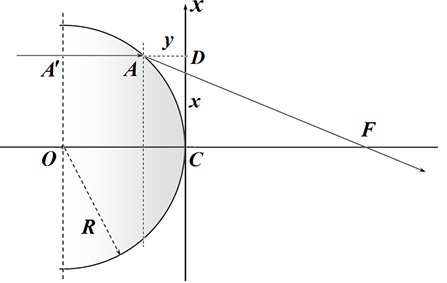
\includegraphics[width=0.45\textwidth]{Figures/P3/Fig 3.2S.png}
\end{wrapfigure}

\noindent\textbf{2.} Lập luận tương tự ý trước điều kiện tồn tại của tiêu điểm là: thời gian mà ánh sáng đi qua khoảng cách $AF + A'A$ không phụ thuộc vào khoảng cách $x$ từ tia sáng đến quang trục. Giả sử ánh sáng truyền đi một khoảng cách $ l $ trong môi trường đồng nhất có chiết suất $ n $, khi đó thời gian truyền bằng:
\begin{equation}
  \label{eq:39}
  t = \frac{l}{c/n} = \frac{nl}{c}
\end{equation}
với $c/n $ là tốc độ ánh sáng trong môi trường này. Lưu ý rằng thay vì tính toán sự thay đổi của tốc độ ánh sáng (điều thực sự xảy ra), khi tính toán thời gian truyền, ta có thể coi tốc độ ánh sáng không đổi (và bằng tốc độ ánh sáng trong chân không $ c $) nhưng độ dài đường truyền tăng lên thành $ nl $ (trong quang học, đại lượng này được gọi là độ dài đường đi quang học). Do đó, điều kiện tồn tại của tiêu điểm là đẳng thức sau được thỏa mãn với mọi giá trị của $ x $:
\begin{equation}
  \label{eq:310}
  n(R-y)+\sqrt{x^{2}+(f+y)^{2}}=nR+f
\end{equation}
biến đổi ta được:
\begin{equation}
  \label{eq:311}
  \sqrt{x^{2}+(f+y)^{2}}=f+ny\implies x^{2}+f^{2}+2fy+y^{2}=f^{2}+2fny+n^{2}y^{2}\implies x^{2}=2(n-1)fy
\end{equation}
nếu mặt cong của thấu kính được mô tả bằng phương trình:
\begin{equation}
  \label{eq:312}
  y = \frac{x^{2}}{2(n - 1)f}
\end{equation}
thì đẳng thức \eqref{eq:310} sẽ được thỏa mãn với mọi giá trị của $ x $, tức $ F $ là tiêu điểm. Nhưng hàm này mô tả trong xấp xỉ paraxial một "cung tròn" có bán kính $ R $:
\begin{equation}
  \label{eq:313}
  y = \frac{x^{2}}{2R}
\end{equation}
do đó, thấu kính được mô tả trong điều kiện bài toán có tiêu điểm. Để xác định tiêu cự của thấu kính, ta chỉ cần so sánh các biểu thức \eqref{eq:312} và \eqref{eq:313}, từ đó suy ra rằng tiêu cự này bằng:
\begin{equation}
  \label{eq:314}
  f = \frac{R}{n-1}
\end{equation}

\begin{wrapfigure}[10]{r}{8cm}
  \centering
  \vspace{-8mm}
  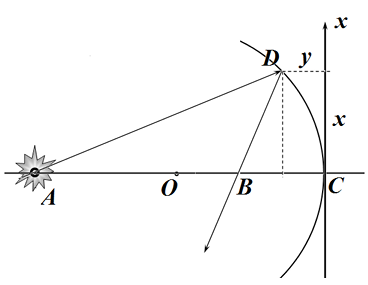
\includegraphics[width=0.4\textwidth]{Figures/P3/Fig 3.3S.png}
\end{wrapfigure}

\noindent\textbf{3a.} Tương tự như các bài toán trước: để tồn tại ảnh tại điểm $B$, khoảng cách $ DB + AD $ không phụ thuộc vào vị trí của điểm $ D $ trên bề mặt gương và bằng khoảng cách $ CB + AC $. Điều kiện này sẽ được thỏa mãn nếu đẳng thức:
\begin{equation}
  \label{eq:315}
  \sqrt{x^{2}+(a-y)^{2}}+\sqrt{x^{2}+(b-y)^{2}}=a+b
\end{equation}
được thỏa mãn với mọi $ x $. Bình phương tổng của các căn thức là một bài toán không đơn giản, vì vậy chúng ta sẽ sử dụng các công thức gần đúng để biến đổi đẳng thức \eqref{eq:315}. Trước tiên, ta sẽ viết lại \eqref{eq:315} dưới dạng:
\begin{equation}
  \label{eq:316}
  \sqrt{x^{2}+(a-y)^{2}}+\sqrt{x^{2}+(b-y)^{2}}\approx \sqrt{x^{2}+a^{2}-2ay}+\sqrt{x^{2}+b^{2}-2by}
\end{equation}
ở đây, ta đã bỏ qua các số hạng $ y^{2} $, nhưng giữ lại các số hạng $ x^{2} $. Trước đó, ta đã chỉ ra rằng đối với đường tròn (và tiếp tuyến parabol), đại lượng $ y $ tỷ lệ với $ x^{2} $, vì vậy các đại lượng này là các số hạng nhỏ cùng bậc. Đại lượng $ y^{2} $ tỷ lệ với $ x^{4} $, do đó có thể bỏ qua nó. Sử dụng mối quan hệ giữa các đại lượng nhỏ này, chúng ta tiếp tục các biến đổi đại số, sử dụng công thức \eqref{eq:p31} được cho trong đề bài:
\begin{equation}
  \label{eq:317}
  \sqrt{x^{2}+a^{2}-2ay}+\sqrt{x^{2}+b^[2]-2by}\approx a+\frac{(x^{2}-2ay)}{2a}+b+\frac{(x^{2}-2by)}{2a}
\end{equation}
thay vào \eqref{eq:315}:
\begin{equation}
  \label{eq:318}
  a+\frac{(x^{2}-2ay)}{2a}+b+\frac{(x^{2}-2by)}{2a}=a+b
\end{equation}
từ đó suy ra rằng \eqref{eq:315} sẽ được thỏa mãn với nếu hàm $ y(x) $ có dạng như sau:
\begin{equation}
  \label{eq:319}
  y=\frac{x^{2}}{4a}+\frac{x^{2}}{4b}=\left(\frac{1}{a}+\frac{1}{b}\right)\frac{x^{2}}{4}
\end{equation}
một lần nữa, chúng ta nhận được phương trình của parabol, có thể coi như parabol tiếp tuyến với đường tròn. So sánh biểu thức \eqref{eq:319} với phương trình "parabol" của đường tròn:
\begin{equation*}
  y = \frac{x^{2}}{2R}
\end{equation*}
ta có thể nhận thấy rằng tồn tại một giá trị $ b $, mà đẳng thức (15) được thỏa mãn với mọi tia sáng phát ra từ điểm $ A $. Nghĩa là ảnh của điểm này tồn tại.\\

\noindent\textbf{3b.} Từ \eqref{eq:319} và phương trình "đường tròn", ta có công thức gương cần tìm:
\begin{equation}
  \frac{1}{a}+\frac{1}{b}=\frac{2}{R}=\frac{1}{f}
\end{equation}
ở đây, ta đã sử dụng giá trị tiêu cự đã nhận được trước đó $ f = \dfrac{R}{2} $.\\

\noindent\textbf{4a.} Trong trường hợp này, các tia sáng xuất phát từ điểm $A$ và phản xạ từ gương sẽ không giao nhau. Nhưng chúng có thể giao nhau tại một điểm kéo dài của các tia phản xạ. Giả sử rằng để kéo dài các tia, khoảng cách phải được coi là âm. \\

\begin{wrapfigure}[10]{r}{8cm}
  \centering
  \vspace{-8mm}
  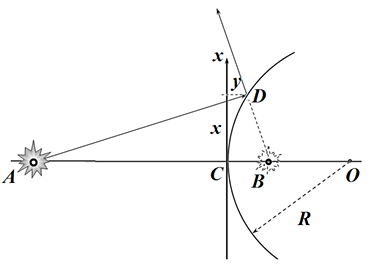
\includegraphics[width=0.42\textwidth]{Figures/P3/Fig 3.4S.png}
\end{wrapfigure}

\noindent\textbf{4b.} Trong khuôn khổ giả định này, điều kiện tồn tại của ảnh ảo được phát biểu như sau: khoảng cách $DB-AD$ là như nhau đối với tất cả các tia phản xạ từ gương, và bằng $CB-AC=b-a$. Điều kiện này được viết dưới dạng đẳng thức, tương tự như (15):
\setcounter{equation}{19}
\begin{equation}
  \label{eq:320}
  \sqrt{x^{2}+(a+y)^{2}}-\sqrt{x^{2}+(b-y)^{2}}=a-b
\end{equation}
biến đổi ta được:
\begin{align}
  \label{eq:321}
   & \sqrt{x^{2}+(a+y)^{2}}-\sqrt{x^{2}+(b-y)^{2}}\approx\sqrt{x^{2}+a^{2}+2ay}-\sqrt{x^{2}+b^{2}-2by}                                 \\
   & \approx \left(a+\frac{x^{2}+2ay}{2a}\right)-\left(b+\frac{x^{2}-2by}{2b}\right)=a-b\implies\frac{x^{2}}{2a}-\frac{x^{2}}{ab}+2y=0
\end{align}
sử dụng "phương trình parabol" của đường tròn:
\begin{equation*}
  y=\frac{x^{2}}{2R}
\end{equation*}
ta có:
\begin{equation}
  \label{eq:322}
  \frac{1}{a}-\frac{1}{b}=-\frac{2}{R}
\end{equation}
công thức này tương tự với "công thức gương cầu lõm" nếu:
\begin{itemize}
  \item Khoảng cách đến ảnh ảo là âm;
  \item Tiêu cự cũng phải là âm $f=-\frac{R}{2}$.
\end{itemize}

\noindent\textbf{4c.} Quang học hình học là một xấp xỉ của quang học sóng. Do đó, nguyên lý đẳng thời có thể được giải thích như sau:
\begin{itemize}
  \item Mỗi tia sáng có thể tương ứng với một sóng nào đó;
  \item  Nếu tất cả các sóng này đi từ nguồn đến ảnh trong cùng một thời gian, thì các pha của chúng là giống nhau;
  \item  Kết quả là tại điểm ảnh sẽ xảy ra sự giao thoa với cường độ tối đa.
\end{itemize}

\subsection*{Phần 3: Nguyên lý Fermat}
\begin{wrapfigure}[6]{r}{8cm}
  \centering
  \vspace{-12mm}
  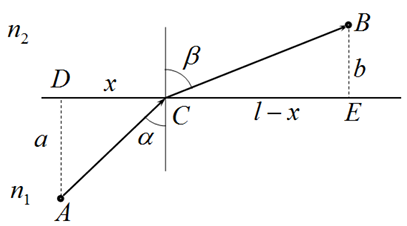
\includegraphics[width=0.4\textwidth]{Figures/P3/Fig 3.5S.png}
\end{wrapfigure}

\noindent\textbf{1.} Giả sử tia sáng đi từ điểm $A$ đến điểm $B$ (xem hình), khúc xạ tại ranh giới giữa hai môi trường tại điểm $C$. Vị trí của điểm này được xác định bởi khoảng cách $x$ tính từ điểm $D$. Đặt $DE=l$, khi đó $CE=l-x$. Thời gian di chuyển của ánh sáng theo đường $ACB$ bằng:
\begin{equation}
  \label{eq:323}
  \tau(x)=\frac{\sqrt{a^{2}+x^{2}}}{c/n_{1}}+\frac{\sqrt{b^{2}+(l-x)^{2}}}{c/n_{2}}=\frac{n_{1}\sqrt{a^{2}+x^{2}}+n_{2}\sqrt{b^{2}+(l-x)^{2}}}{c}
\end{equation}
theo nguyên lý Fermat, khi di chuyển theo quỹ đạo thực, thời gian này là nhỏ nhất, tức ta phải tìm cực trị của hàm \eqref{eq:323}
\begin{equation}
  \label{eq:324}
  \tau'(x)=\frac{2n_{1}x}{2\sqrt{a^{2}+x^{2}}}-\frac{2n_{2}(l-x)}{2\sqrt{b^{2}+(l-x)^{2}}}=0
\end{equation}
từ hình vẽ, ta có:
\begin{equation}
  \label{eq:325}
  \sin{\alpha}=\frac{x}{\sqrt{a^{2}+x^{2}}}, \quad \sin{\beta}=\frac{l-x}{\sqrt{b^{2}+(l-x)^{2}}}
\end{equation}
do đó, từ \eqref{eq:324} và \eqref{eq:325}, suy ra định luật khúc xạ ánh sáng:
\begin{equation}
  \label{eq:326}
  n_{1}\sin{\alpha}=n_{2}\sin{\beta}
\end{equation}

\begin{wrapfigure}[5]{r}{5.5cm}
  \centering
  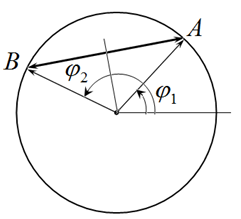
\includegraphics[width=0.25\textwidth]{Figures/P3/Fig 3.6S.png}
\end{wrapfigure}

\noindent\textbf{2a.} Để tính độ dài của quỹ đạo, ta sẽ sử dụng công thức đơn giản cho độ dài dây cung $l$ của $AB$, được viết tổng quát như sau:
\begin{equation}
  \label{eq:327}
  l=2R\lvert\sin\frac{\varphi_{1}-\varphi_{2}}{2}\rvert
\end{equation}
\begin{figure}[h]
  \centering
  \vspace{1cm}
  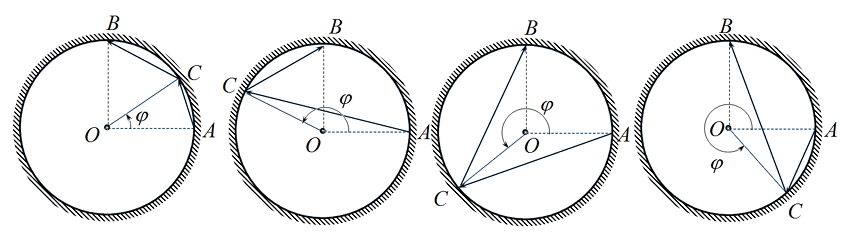
\includegraphics[width=1\textwidth]{Figures/P3/Fig 3.7S.png}
\end{figure}

\noindent độ dài quỹ đạo tia sáng với một lần phản xạ từ bề mặt trong $ACB$ bằng tổng độ dài của hai dây cung, do đó có thể được mô tả bằng công thức:
\begin{equation}
  \label{eq:328}
  L=2R\left(\sin\frac{\varphi}{2}+\lvert\sin\left(\frac{\varphi}{2}-\frac{\pi}{4}\right)\rvert\right)
\end{equation}
viết lại công thức này cho hai khoảng giá trị của góc $\phi$, khi $\phi \leqslant \dfrac{\pi}{2}$:
\begin{equation}
  \label{eq:329}
  L=2R\sin\frac{\varphi}{2}+2R\sin\frac{\pi/2-\varphi}{2}=4R\sin\frac{\pi}{8}\cos\left(\frac{\pi}{8}-\frac{\varphi}{2}\right)
\end{equation}
khi $\varphi\geqslant\dfrac{\pi}{2}$:
\begin{equation}
  \label{eq:330}
  L=2R\sin\frac{\varphi}{2}+2R\sin\frac{\varphi-\pi/2}{2}=4R\sin\left(\frac{\varphi}{2}-\frac{\pi}{8}\right)\cos\left(\frac{\pi}{8}\right)
\end{equation}

\noindent Đồ thị biểu diễn sự phụ thuộc này được chỉ ra trên hình:
\begin{figure}[h]
  \centering
  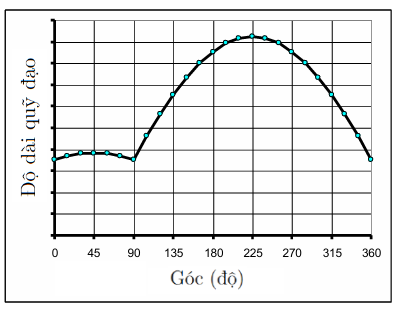
\includegraphics[width=0.6\textwidth]{Figures/P3/Fig 3.8S.png}
\end{figure}

\noindent\textbf{2b.} Các quỹ đạo thực của tia sáng thỏa mãn định luật phản xạ ánh sáng xảy ra khi:
\begin{equation}
  \label{eq:331}
  \varphi=\begin{cases}
    \dfrac{\pi}{4} \\
    \dfrac{\pi}{4}+\pi=\dfrac{5\pi}{4}
  \end{cases}
\end{equation}
với các giá trị này, độ dài của quỹ đạo là tối đa.\\

\noindent\textbf{3a.} Nguyên lý Fermat có thể được hiểu như sau: ánh sáng chọn từ nhiều con đường giữa hai điểm ra một con đường đòi hỏi thời gian cực trị (tối thiểu hoặc tối đa) hoặc thời gian tĩnh (không phụ thuộc vào quỹ đạo). Về mặt toán học, nguyên lý này được phát biểu như sau: Giả sử chiều dài của quỹ đạo được mô tả bởi một hàm số của tham số $\xi$, xác định quỹ đạo, $L(\xi)$. Khi đó, các quỹ đạo thực tương ứng với các giá trị tham số $\xi^*$, mà tại đó đạo hàm của hàm số bằng không:
\begin{equation}
  \label{eq:332}
  L'(\xi^*)=0
\end{equation}

\noindent\textbf{3b.} Giải thích nguyên lý Fermat xuất phát từ tính chất sóng của ánh sáng. Trong phạm vi lân cận điểm cực trị, khi tham số thay đổi từ giá trị tĩnh $\xi^*$ một lượng nhỏ $\Delta\xi$, chiều dài của quỹ đạo sẽ thay đổi một lượng tỉ lệ với $(\Delta\xi)^2$. Do đó, gần điểm cực trị có một phạm vi rộng của các quỹ đạo mà chiều dài của chúng thay đổi một lượng rất nhỏ. Các sóng lan truyền dọc theo những quỹ đạo này đến điểm quan sát với độ lệch pha, do đó thỏa mãn điều kiện cực đại của giao thoa.
























\end{document}